\documentclass[12 pt]{article}
\usepackage{graphicx} % Required for inserting images
\usepackage[a4paper, inner= 1.5in, outer= 1in, top= 1in, bottom= 1in]{geometry}
\usepackage[onehalfspacing]{setspace} % to create a half spacing of 1.5 in
% \thispagestyle{}
\usepackage{ragged2e}
\usepackage{times}
\usepackage{fancyhdr}

\fancyhf{}
\pagenumbering{arabic}

\begin{document}
%%%%%%%%%%%%%%%%%%%% Title page %%%%%%%%%%%%%%%%%%%%%%%%%%%
\begin{center}

    \thispagestyle{empty}
    {\fontsize{16 pt}{12} \selectfont\textbf{TRIBHUVAN UNIVERSITY} \\
        \textbf{INSTITUTE OF ENGINEERING}} \\
    \vspace{0.3 in}

    
\includegraphics[width= 4in ]{leclogo21.png} \\
    \vspace{0.05 in}
    LALITPUR ENGINEERING COLLEGE \\
    KHOLKA POKHARI, LALITPUR \\

    \vspace{0.5 in}
    \textbf{ A PROPOSAL OF MAJOR PROJECT}\\
    {\fontsize{14 pt}{12} \selectfont \textbf{ITHUB}}\\
    \vspace{1.1 in}
    \textbf{ SUBMITTED BY}  \\
    ABHISHEK NEUPANE (LEC-076-BCT-02)   \\
    RABINDRA ADHIKARI (LEC-076-BCT-025) \\
    SANJISH MAHARJAN (LEC-076-BCT-032)  \\
    SUSHIL KAFLE (LEC-076-BCT-045)  \\
    \vspace{1.1 in}
    \textbf{ SUBMITTED TO}  \\
    DEPARTMENT OF COMPUTER ENGINERING \\
    \vspace{0.5 in}
    \textbf{Date} \\
\end{center}
\newpage

\begin{center}
    \pagenumbering{Roman}
    \section*{ABSTRACT}
    \justify
    Deepfakes are realistic-looking fake media generated by deep-learning algorithms that iterate through large datasets until
    they have learned how to solve the given problem (i.e., swap faces or objects in video and digital content). The massive generation
    of such content and modification technologies is rapidly affecting the quality of public discourse and the safeguarding of
    human rights. Deepfakes are being widely used as a malicious source of misinformation in court that seek to sway a court’s decision.
    Because digital evidence is critical to the outcome of many legal cases, detecting deepfake media is extremely important and in high demand in digital forensics.
    As such, it is important to identify and build a classifier that can accurately distinguish between authentic and disguised media, especially in facial-recognition systems
    as it can be used in identity protection too. In this work, we compare the most common, state-of-the-art face-detection classifiers such as Custom CNN, VGG19, and DenseNet-121
    using an augmented real and fake face-detection dataset. Data augmentation is used to boost performance and reduce computational resources. Our preliminary results indicate that VGG19 has the best performance
    and highest accuracy of 95\% when compared with other analyzed models.\\
    \vspace{3 in}
    \\ \textit{Keywords: deepfake detection; digital forensics; media forensics; deep learning; VGG19; face-image manipulation}

    \newpage

    \tableofcontents
    \thispagestyle{empty}
    \newpage
    \listoffigures
\end{center}
\newpage
\pagenumbering{arabic}
\section{INTRODUCTION}
In the last few years, cybercrime, which accounts for a 67\% increase in the incidents of security breaches, has been one of the most challenging problems that national security systems have had to deal with worldwide [1].
Deepfakes (i.e., realistic-looking fake media that has been generated by deep-learning algorithms) are being widely used to swap faces or objects in video and digital content. This artificial intelligence-synthesized
content can have a significant impact on the determination of legitimacy due to its wide variety of applications and formats that deepfakes present online (i.e., audio, image and video).
Considering the quickness, ease of use, and impacts of social media, persuasive deepfakes can rapidly influence millions of people, destroy the lives of its victims and have a negative impact on society in general [1].
\\ The generation of deepfake media can have a wide range of intentions and motivations, from revenge porn to political fake news..
Deepfakes have also been published to falsify satellite images with non-existent landscape features for malicious purposes [3].
There are numerous captivating applications of deepfakery in video compositing and transfiguration in portraits, especially in identity protection as it can replace faces in photographs with ones from a collection of stock images.
Cyber-attackers, using various strategies other than deepfakery, are always aiming to penetrate identification or authentication systems to gain illegitimate access. Therefore, identifying deepfake media using forensic methods remains
an immense challenge since cyber-attackers always leverage newly published detection methods to immediately incorporate them in the next generation of deepfake generation methods. With the massive usage of the Internet and social media,
and billions of images available on the Internet, there has been an immense loss of trust from social media users. Deepfakes are a significant threat to our society and to digital evidence in courts. Therefore, it is highly important to
obtain state-of-the-art techniques to identify deepfake media under criminal investigation.
As demonstrated in Table 1 (inspired by the figure presented in [1]), tampering of evidence, scams and frauds (i.e., fake news), digital kidnapping associated with ransomware blackmailing, revenge porn and political sabotage are among the
vast majority of types of deepfake activities with the highest level of intention to mislead [1].
\newpage
\subsection{Background}
\newpage
\subsection{Problem Statement}
\newpage
\subsection{Objectives}
\justify
\begin{itemize}
    \item Our project aims at discovering the distorted truth of the deep fakes.
    \item Our project will reduce the Abuses’ and misleading of the common people on
          the world wide web.
    \item Our project will distinguish and classify the video as deepfake or pristine.
    \item Provide a easy to use system for used to upload the video and distinguish
          whether the video is real or fake
\end{itemize}
\newpage
\subsection{Scope}
Our deepfake detection project aims to provide a web-based platform for users to upload videos and classify them as either fake or real. The platform will serve as a valuable tool in preventing the proliferation of deepfakes on the internet. Additionally, we envision the potential to scale up the project by developing a browser plugin for automatic deepfake detection. This would enable seamless integration with popular applications such as WhatsApp and Facebook, allowing users to detect deepfakes before sharing them with others.
The system will support video uploads of varying sizes, ranging from small video clips to larger files. The exact size limit will depend on the implementation and infrastructure constraints. However, efforts will be made to accommodate a wide range of video sizes to ensure user convenience.
\newpage


\section{LITERATURE REVIEW}
\newpage
\subsection{Existing Systems}
\newpage
\subsection{Proposed Systems}
\newpage


\section{FEASIBILITY STUDY}
\subsection{Economic feasibility}
This is a low-budget project with no development costs. The total expenditure of the
project is just computational power. The dataset and computational power required for
the project are easily available. The computational power is easily provided by google
collab. So, the project is economically feasible. The system will be simple to
comprehend and use. As a result, there will be no need of trained personnel to use the
system. This system will have the capacity to expand by adding more components.
\subsection{Operational feasibility}
\subsection{Technical feasibility}
The purpose of technical feasibility is to establish whether the project is possible in
terms of software, hardware, manpower, and knowledge to complete. It will take into
account determining resources in support of the suggested scheme. The system is
platform independent because it is written in Python. Advanced machine learning
libraries are available and the technology is cutting-edge. As a result, the system is
technically possible.
\newpage

\section{METHODOLOGY}
\subsection{Software Development Life Cycle}
\justify
Agile method of Software Development uses iterative approach. Agile method cycles
among Planning, Requirement Analysis, Designing, Development and Testing stages.
These cycle is called sprints. Each sprints are considered as a miniature project on itself.
Using this method allowed us to update various parts of project at any point of project
development. In this model an iterative approach was taken where working software
was delivered after each iteration some new features is added to main system. It works
in incremental and iterative approach. Agile model mainly focuses on customer
collaborations, on individuals and iterations and welcomes changes at anytime in
SDLC process. We prefer to use agile model in this system as it helps in developing
realistic systems and promotes teamwork during software development. Also system is
easy to manage and it can accommodate new changes at any stages of software
development phase. \\
\vspace{0.2 in}
\begin{figure}[h]
    \centering
    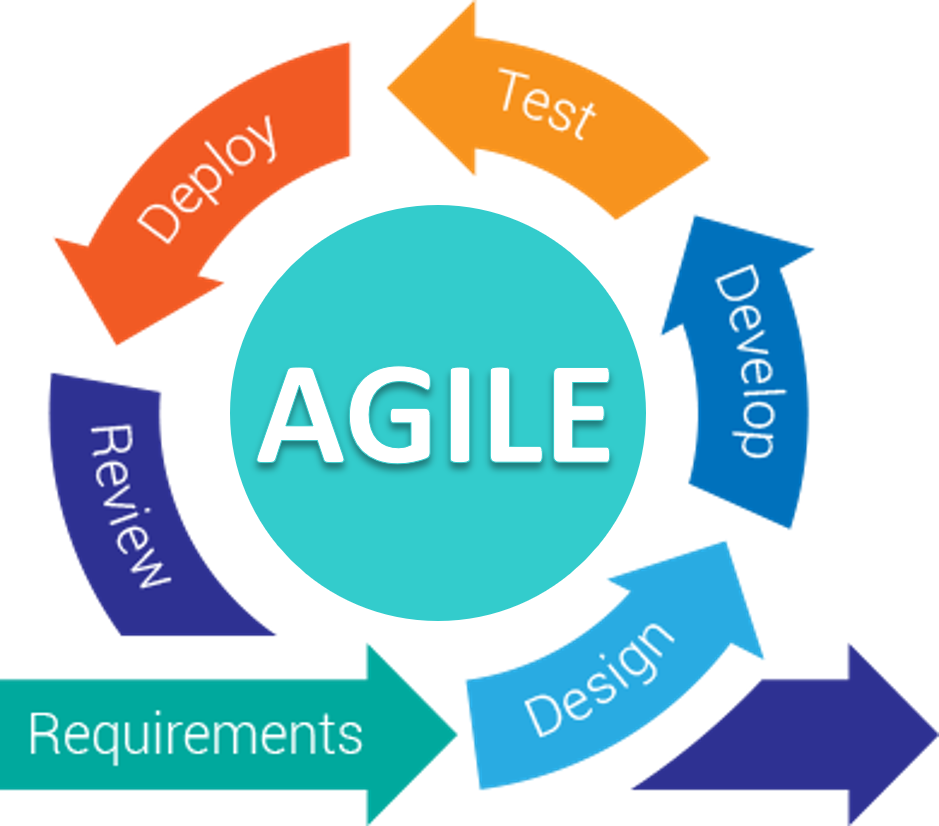
\includegraphics[width= 3in ]{agile.png}
    \caption{Agile Model}
\end{figure}

\newpage
\subsection{System Development Tools}
Our static Deepfake detection System requires Python, Tensorflow, OpenCV,
Machine Learning which are listed below:
\begin{enumerate}
    \item Python
    \item Pytorch
    \item NumPy
    \item OpenCV
    \item Tensorflow
\end{enumerate}
\subsection{Functional Requirement}
The functional requirements of the system are:
\begin{enumerate}
    \item Detecting the Faces from Images and Videos.
    \item Testing for realism of image.
\end{enumerate}

\subsection{Non Functional Requirement}
\justify
These requirements are not needed by the system but are essential for the better
performance of software. The points below focus on the non-functional requirement of
the system.
\begin{itemize}
    \item Reliability
    \item   Usability
    \item   Security
    \item   Portability
    \item   Speed and responsiveness
    \item  Performance
\end{itemize}


\newpage

\section{BLOCK DIAGRAMS}
\newpage
\subsection{System Architecture}
\newpage
\subsection{System Design}
\newpage
\subsection{Use Case Diagram}
\newpage
\subsection{Sequence Diagram}
\newpage
\subsection{Class Diagram}
\newpage
\subsection{Dataflow Diagram}
\newpage
\subsection{Activity Diagram}
\newpage


\section{EXPECTED OUTCOMES}
\begin{itemize}
    \item User-friendly interface for easy upload and clear result presentation.
    \item Accurate identification of manipulated media content.
    \item Robust performance against different deepfake techniques and adversarial attacks.
\end{itemize}
\newpage
\section{LIMITATIONS}
\begin{itemize}
    \item Deepfake detection projects face challenges due to rapidly evolving techniques and the need for diverse training data.
    \item Adversarial attacks can exploit weaknesses in detection algorithms, making deepfakes harder to identify accurately.
    \item Deepfake detection algorithms often require significant computational resources, limiting their applicability on resource-constrained devices.
\end{itemize}
\newpage
\section{FUTURE ENHANCEMENTS}
There is always a scope for enhancements in any developed system, especially
when the project build using latest trending technology and has a good scope in
future.
\begin{itemize}
    \item Web based platform can be upscaled to a browser plugin for ease of access to
          the user.
    \item Currently only Face Deep Fakes are being detected by the algorithm, but the
          algorithm can be enhanced in detecting full body deep fakes.
\end{itemize}
\newpage

\begin{thebibliography}{99}
    \bibitem{1}Andreas Rossler, Davide Cozzolino, Luisa Verdoliva, Christian Riess, Justus
    Thies,Matthias Nießner, “FaceForensics++: Learning to Detect Manipulated Facial
    Images” in arXiv:1901.08971.
    \bibitem{2}Deepfake detection challenge dataset : https://www.kaggle.com/c/deepfake-detection challenge/data Accessed on 26 March, 2020
    \bibitem{3} Yuezun Li , Xin Yang , Pu Sun , Honggang Qi and Siwei Lyu “Celeb-DF: A
    Large-scale Challenging Dataset for DeepFake Forensics” in arXiv:1909.12962
    \bibitem{3}10 deepfake examples that terrified and amused the internet :
    https://www.creativebloq.com/features/deepfake-examples Accessed on 26 March,
    2020
    \bibitem{3}Keras: https://keras.io/ (Accessed on 26 March, 2020)
    \bibitem{3}PyTorch : https://pytorch.org/ (Accessed on 26 March, 2020)
    \bibitem{3}G. Antipov, M. Baccouche, and J.-L. Dugelay. Face aging with conditional generative adversarial networks. arXiv:1702.01983, Feb. 2017
    \bibitem{3} TensorFlow: https://www.tensorflow.org/ (Accessed on 26 March, 2020)
    \bibitem{3}Face app: https://www.faceapp.com/ (Accessed on 26 March, 2020)
    \bibitem{3}Face Swap : https://faceswaponline.com/ (Accessed on 26 March, 2020)

\end{thebibliography}

\end{document}
